\section{Simulation Experiments}
\label{section: simulation}

In addition to the real-world experiments, we use simulation to evaluate performance more comprehensively based on random task sets, 
covering a wider range of system scales and load conditions.
We organize the results into four comparisons, each with its own conclusion:
the gap to the brute-force optimum (Section~\ref{section: sim_vs_optimal}),
performance against baselines and scalability (Section~\ref{section: sim_vs_baselines}),
an ablation of the individual mechanisms (Section~\ref{section: sim_ablation}),
and the effectiveness of the fallback mechanism (Section~\ref{section: sim_fallback}).

\subsection{Simulated Task Sets Generation}
\label{section: sim_task_gen}

In simulation, the robot operates in a 2D square environment of width $W^E$ and height $H^E$,
with $W^E = H^E = 200$ m and a speed of $1.0$ m/s.
Task sets follow the standard real-time-systems experimental design~\cite{Wang2023RTAS, Zhao2020AnOF}
based on Uunifast~\cite{Davis2008EfficientES}.
Each set comprises $N$ tasks on $2$ CPU cores under partitioned scheduling,
with $N \in \{4, 6, 8, 10, 12, 14, 16\}$; for each $N$ we generate $10$ independent task sets
and aggregate the results.
Periods are drawn from $\{20, 33, 50, 100, 200, 500, 1000\}$ ms~\cite{Percept21_RTSS, Kramer15benchmark}.
Per-core utilization is drawn from $U[0.5, 1.0]$---where $U[a,b]$ denotes the uniform distribution on
$[a,b]$---and distributed across tasks by Uunifast to set each task's mean execution time
$\mu^E_{c,i}$; all tasks use implicit deadlines $D_i = T_i$.

Each task is one of the types defined in Section~\ref{section: system_model_tasks}, assigned in three groups.
First, we designate $N_{\text{env}} = \lceil \rho_{\text{env}} \cdot N \rceil$ tasks as environment-dependent
tasks $\tau^E_i$ with spatial variation; here $\rho_{\text{env}}$ is the environment-dependent fraction,
drawn from $U[0.1, 0.3]$ and clamped so that $N_{\text{env}} \ge 1$.
Each of the remaining tasks independently becomes a QoS-configurable task $\tau^Q_i$ with probability $0.5$.
The execution time of the rest of the tasks does not change.

We model each task's execution-time distribution according to its type.
For an environment-dependent task, the dependence on the environmen, \ie the robot's location, is captured by a
Gaussian Mixture Model (GMM).
The robot's location $(x, y)$ and a task's execution time $\extDist{i}$ jointly follow a 3D Gaussian;
the per-task distribution is a mixture of $K{=}4$ components (each weighted, floored at $0.1$), with density
\begin{equation}
    f^{E}(x, y, \extDist{i}) =\mathcal{N}(\boldsymbol{\mu}^E, \boldsymbol{\Sigma}^E)
    \label{eq: pdf_gmm}
\end{equation}
\begin{equation}
    \boldsymbol{\mu}^E = \begin{bmatrix}
        \mu^E_x & \mu^E_y & \mu^E_{c,i}
    \end{bmatrix}
\end{equation}
\begin{equation}
    \boldsymbol{\Sigma}^E =
    \begin{bmatrix}
        \sigma_x^2 & 0 & \rho_{x,c,i} \sigma_x \sigma_{c,i} \\
        0 & \sigma_y^2 & \rho_{y,c,i} \sigma_y \sigma_{c,i} \\
        \rho_{x,c,i} \sigma_x \sigma_{c,i} & \rho_{y,c,i} \sigma_y \sigma_{c,i} & \sigma_{c,i}^2
    \end{bmatrix}
\end{equation}

Placing the coordinate origin at the square's center and requiring 95\% coverage gives
$\mu^E_x = \mu^E_y = 0$ and $\sigma_x = W^E/4$, $\sigma_y = H^E/4$.
The mean execution time $\mu^E_{c,i}$ comes from Uunifast.
The environment-dependent tasks' minimum execution time is capped at a per-task utilization of $0.27$ to leave headroom so that spatial
variation does not push the maximum possible execution time above the period near the map boundary.
Their standard deviation is $\sigma_{c,i} = k\,\mu^E_{c,i}$ with $k$ drawn from $U[0.3, 0.4]$, and their
covariance ratios are nonzero: $\rho_{x,c,i}$ is drawn from $U[-0.9, -0.7]$ and $\rho_{y,c,i}$ from
$U[-0.1, 0.1]$, per mixture component. 
These parameters are either measured from our previous real-world experiments, 
or derived to ensure the task set is schedulable under the worst-case scenario if given an optimal scheduling algorithm.
The location-independent environment-dependent tasks use the same GMM but with zero spatial correlation
($\rho_{x,c,i} = \rho_{y,c,i} = 0$), so their distribution does not vary with the robot's location;
their marginal execution-time bounds are $\mu^E_{c,i} \pm 2\sigma_{c,i}$.
A QoS-configurable task's execution time is instead decided by its QoS budget rather than by the
environment: the budget is drawn from a grid of $10$ options spanning $[0.05, 0.9] \times T_i$, and the
execution time is near-deterministic ($\sigma_{c,i} = 0.001\,\mu^E_{c,i}$), so its bounds span the
budget grid.

Each task also carries two SP-specific parameters: its importance weight $w_i$, drawn from $U[0.1, 1.0]$
(then normalized so $\sum_i w_i = 1$), and its deadline-miss threshold $\Theta_i$, drawn from
$U[0.001, 0.9]$ (Section~\ref{section_config_opt}).
The important-task subset $\boldsymbol{\tau}^{safe}$ is the top $50\%$ of tasks by weight, $\lceil 0.5 N \rceil$
tasks, modeling safety-critical tasks shielded from overload.
Tasks are assigned to cores by a worst-fit heuristic to balance load across the two cores.

We evaluate two configurations for the number of tasks in task sets.
The \emph{main} configuration scales to large task sets: $N \in \{4,\dots,16\}$, $600$~s per run,
re-optimization every $10$~s, and a $1$~s optimization budget per scheduler activation
(base seed $1000$, advanced per task set).
The \emph{optimality} configuration isolates the gap to the brute-force optimum at small $N$:
$N \in \{4,6,8\}$, $100$~s horizon, $100$~s interval, and a generous $500$~s optimization budget so that
brute force can fully enumerate the joint priority-and-QoS space.
All SP values are computed with the precise numerical response-time analysis rather than the pessimistic
analytical bound, so the reported SP reflects achievable schedulability.

\subsection{Compared Methods}
\label{section: sim_compared_methods}

We evaluate the same five methods introduced in Section~\ref{section: exp_methods}:
CFS, DM\_FAST, DM\_SLOW, BF, and INCR.
The proposed arm is INCR\_Reopt\_10, the incremental optimizer that re-optimizes from
scratch every $10$ intervals and otherwise optimizes incrementally.
The ablation arms that isolate individual mechanisms of the proposed optimizer
are introduced in Section~\ref{section: sim_ablation}.

\subsection{Comparison Against the Optimal Solution}
\label{section: sim_vs_optimal}

We first ask how close the incremental optimizer comes to the brute-force optimum.
To make BF a valid optimality reference, the optimality configuration gives it a $500$~s budget---enough
to enumerate the joint space at small $N$---while INCR keeps its standard online budget;
the comparison also includes INCR\_Reopt\_1, which re-optimizes from scratch every interval.
Table~\ref{tab_sim_vs_optimal} reports the normalized SP, the SP gap to BF, the optimizer
execution time, and the speedup of INCR over BF.
INCR tracks BF closely: the SP gap is $0.2\%$ at $N{=}4$, $1.7\%$ at $N{=}6$, and $2.1\%$ at
$N{=}8$, never exceeding $2.1\%$.
The price BF pays for this near-optimality is steep: its optimization time grows from $0.09$~s
($N{=}4$) to $32$~s ($N{=}6$) and $423$~s ($N{=}8$), while INCR stays at $0.003$--$0.012$~s,
three to four orders of magnitude faster.
Beyond $N{=}8$ BF becomes intractable, which is why the large-scale study below uses the baseline
schedulers rather than BF as the reference.

\begin{table*}[htbp]
\centering
\caption{Comparison against the brute-force optimum ($N\in\{4,6,8\}$, $500$~s BF budget).
INCR reaches within $2.1\%$ of BF's SP at three to four orders of magnitude lower optimization cost.}
\label{tab_sim_vs_optimal}
\footnotesize
\begin{tabular}{@{}ccccccc@{}}
\toprule
$N$ & BF SP & INCR SP & SP Gap & BF Time (s) & INCR Time (s) & Speedup \\
\midrule
4 & 0.933 & 0.932 & 0.2\% & 0.094 & 0.0028 & $3.4\times10^{1}$ \\
6 & 0.792 & 0.779 & 1.7\% & 32.28 & 0.0048 & $6.7\times10^{3}$ \\
8 & 0.758 & 0.742 & 2.1\% & 423.5 & 0.0117 & $3.6\times10^{4}$ \\
\bottomrule
\end{tabular}
\end{table*}

The incremental optimizer attains near-optimal SP (within $2.1\%$ of brute force) at a fraction of the
computational cost, making it deployable online where exhaustive search is infeasible.

\subsection{Comparison Against Baselines and Scalability}
\label{section: sim_vs_baselines}

The main configuration evaluates INCR against the baseline schedulers across $N \in \{4,\dots,16\}$.
Fig.~\ref{fig_sim_sp_baselines} reports the normalized SP.
INCR\_Reopt\_10 outperforms every baseline at every scale.
At $N{=}4$ it reaches $0.929$, ahead of DM\_SLOW ($0.813$), CFS ($0.729$), and DM\_FAST ($0.675$).
As $N$ grows and the system becomes overloaded, INCR degrades gracefully to $0.670$ at $N{=}16$,
whereas CFS collapses to $0.331$ and DM\_SLOW to $0.265$.
DM\_FAST is the strongest baseline at large $N$ because its small budgets preserve schedulability under
overload, yet INCR still exceeds it by up to $4\%$.
Note that BF here runs under the same $1$~s online budget, so it degrades sharply for $N \ge 8$
($0.639$ at $N{=}8$, $0.386$ at $N{=}12$); at this scale BF is budget-limited rather than optimal,
which is precisely why the optimality gap is established separately in
Section~\ref{section: sim_vs_optimal}.

\begin{figure}[!htbp]
    \centering
    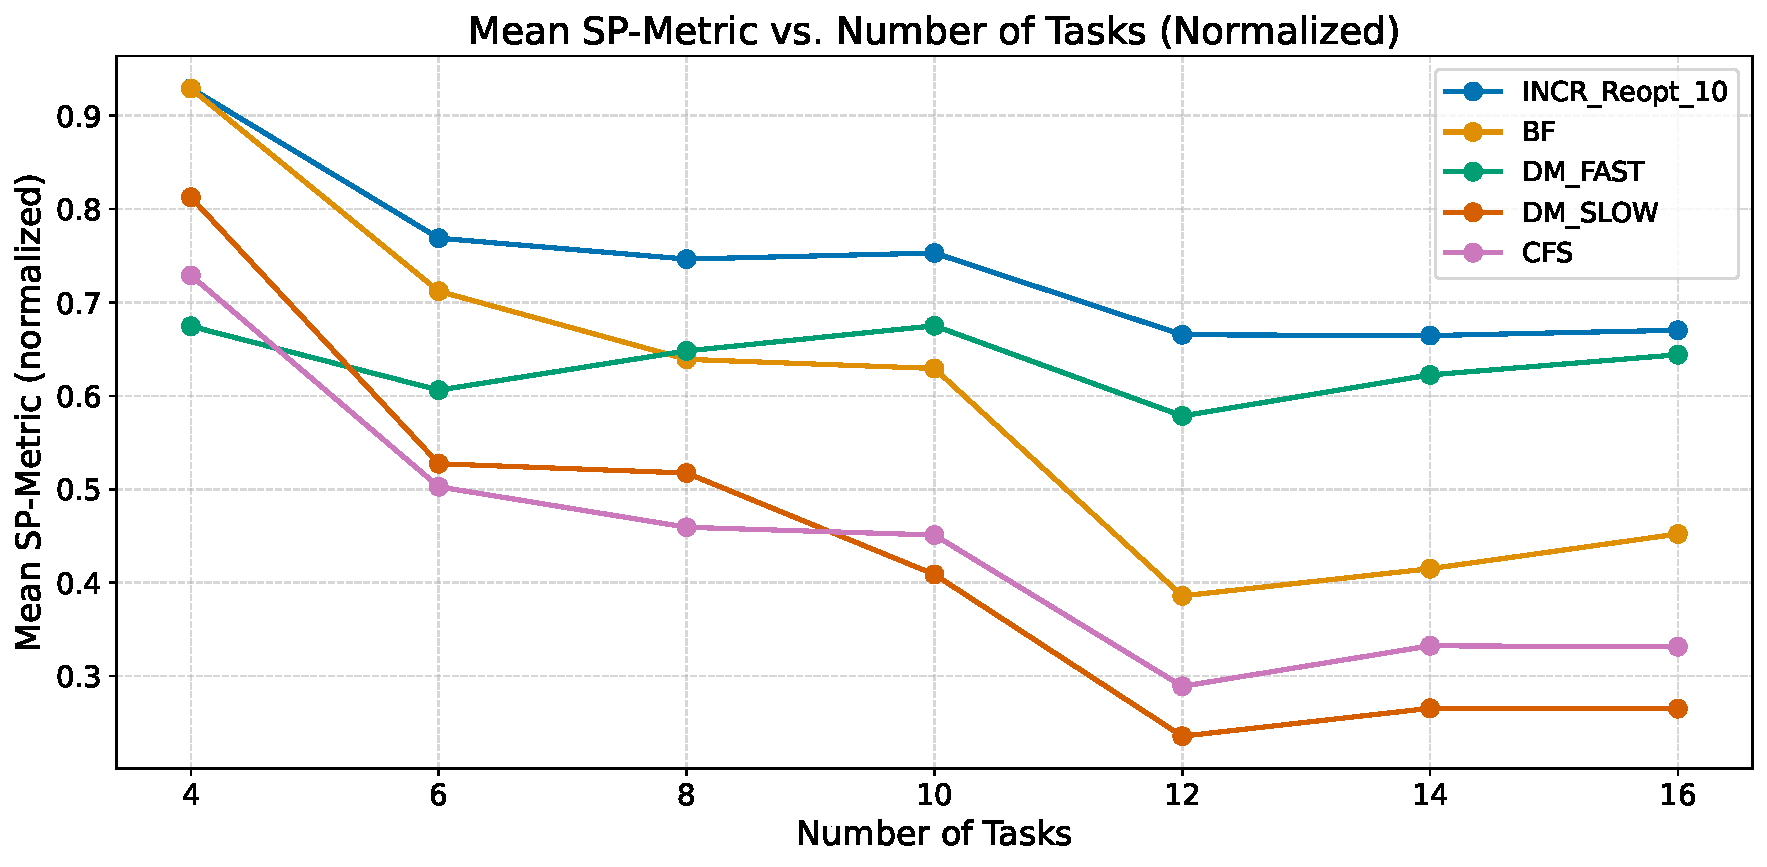
\includegraphics[width=\columnwidth]{pictures/simulation/sim_sp_vs_baselines.pdf}
    \caption{Normalized SP of INCR versus baselines across task count ($N\in\{4,\dots,16\}$).
    INCR dominates all baselines and degrades gracefully under overload.}
    \label{fig_sim_sp_baselines}
\end{figure}

Fig.~\ref{fig_sim_important_miss} reports the deadline-miss rate of the important tasks
$\boldsymbol{\tau}^{safe}$.
INCR keeps this rate below each task's threshold $\Theta_i$ across all $N$, the direct effect of the
in-search important-task feasibility gate (Section~\ref{section_config_opt}).
The baselines, lacking this gate, let important-task misses climb under overload---most steeply for CFS
and DM\_SLOW, whose fixed priorities cannot shield safety-critical work.

\begin{figure}[!htbp]
    \centering
    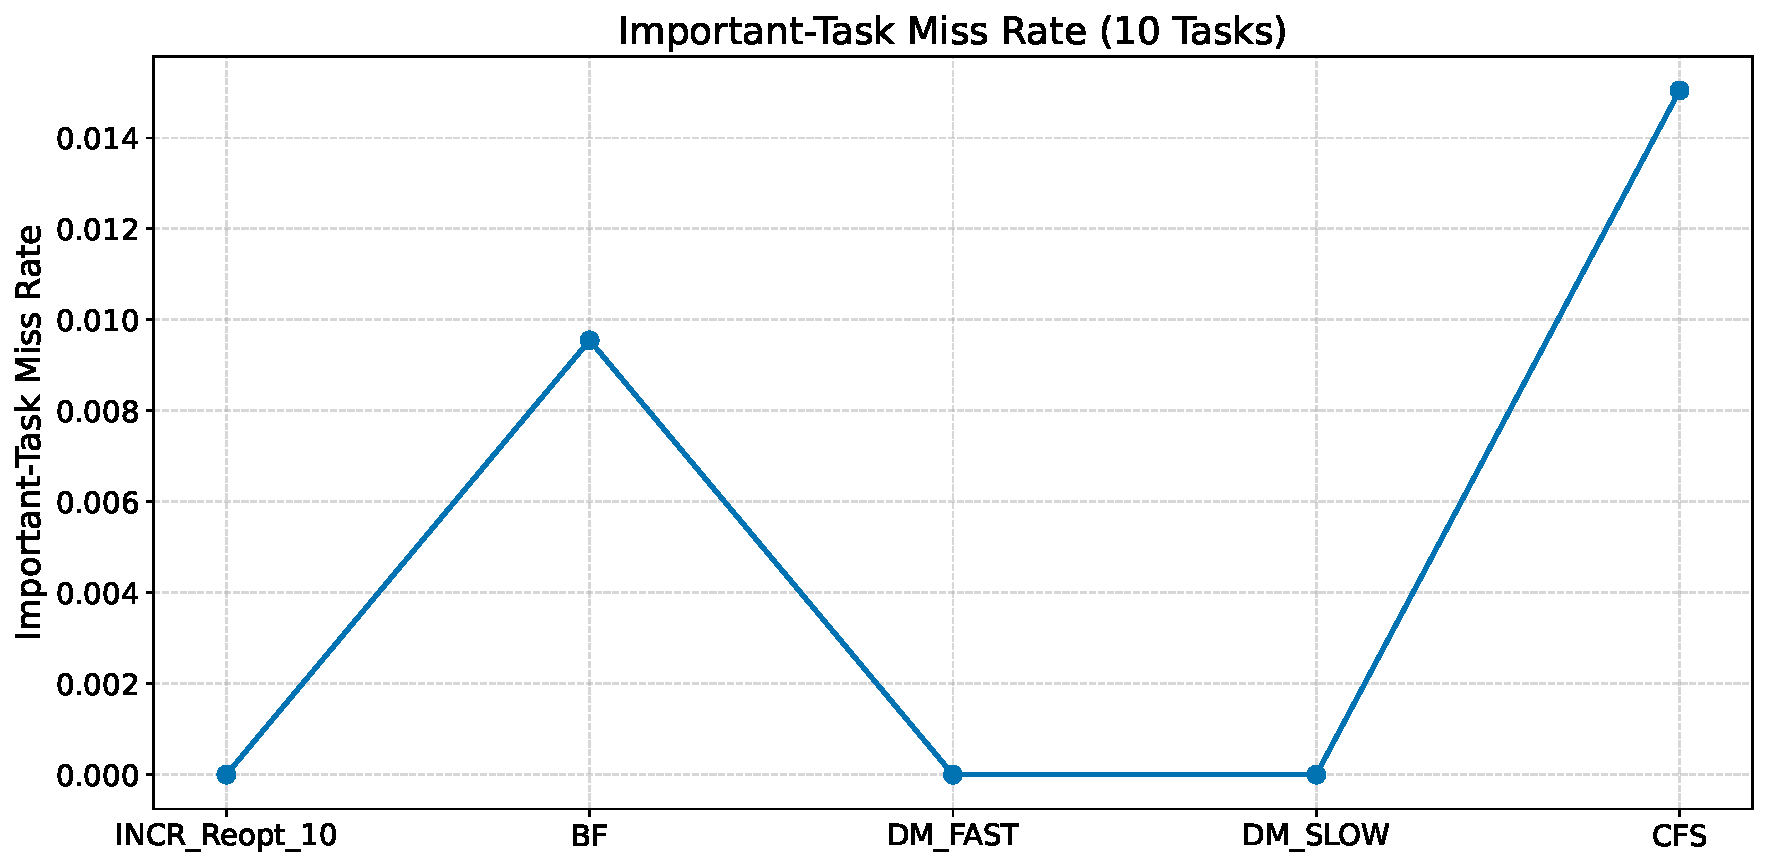
\includegraphics[width=\columnwidth]{pictures/simulation/sim_important_task_miss_rate.pdf}
    \caption{Important-task deadline-miss rate.
    INCR holds the rate below $\Theta_i$ via the in-search feasibility gate; baselines do not.}
    \label{fig_sim_important_miss}
\end{figure}

The optimizer itself stays cheap: INCR's per-activation time grows from $0.005$~s ($N{=}4$) to
$0.126$~s ($N{=}16$), at most $1.3\%$ of the $10$~s interval and well within the $1$~s budget.
INCR thus outperforms all baseline schedulers across the full scale range and keeps important-task
misses bounded, while its online overhead stays below $1.3\%$.

\subsection{Ablation Study}
\label{section: sim_ablation}

\begin{figure*}[!htbp]
    \centering
    \begin{subfigure}[c]{0.48\textwidth}
        \centering
        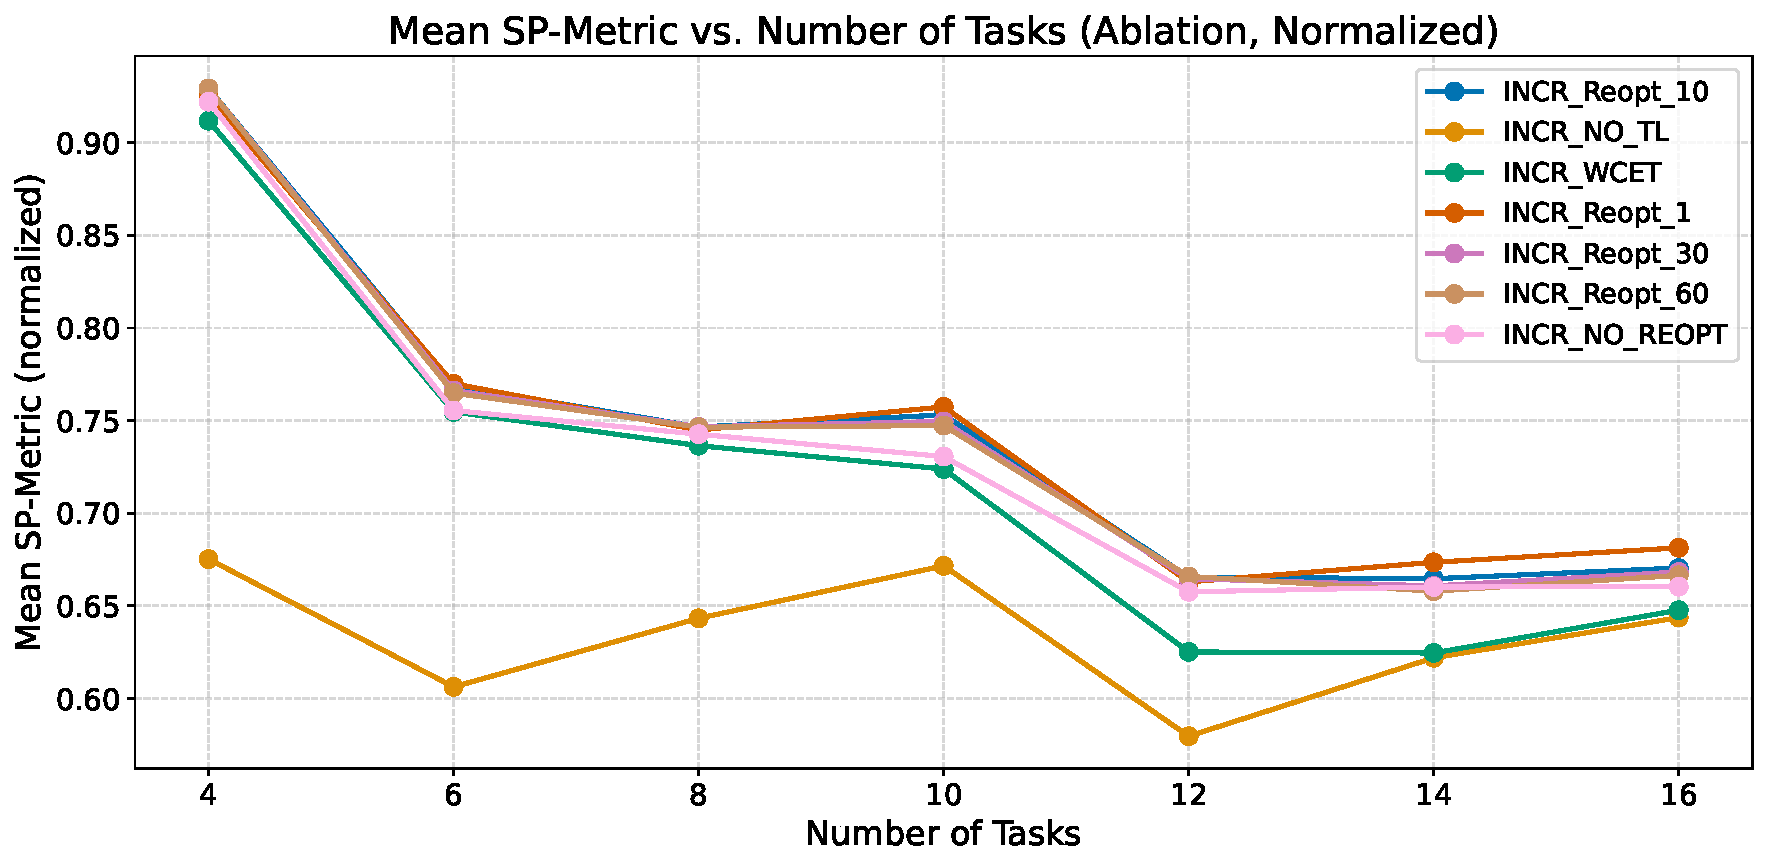
\includegraphics[width=\textwidth]{pictures/simulation/sim_ablation_sp.pdf}
        \caption{Normalized SP of ablation arms.}
        \label{fig_sim_ablation_sp}
    \end{subfigure}\hfill
    \begin{subfigure}[c]{0.48\textwidth}
        \centering
        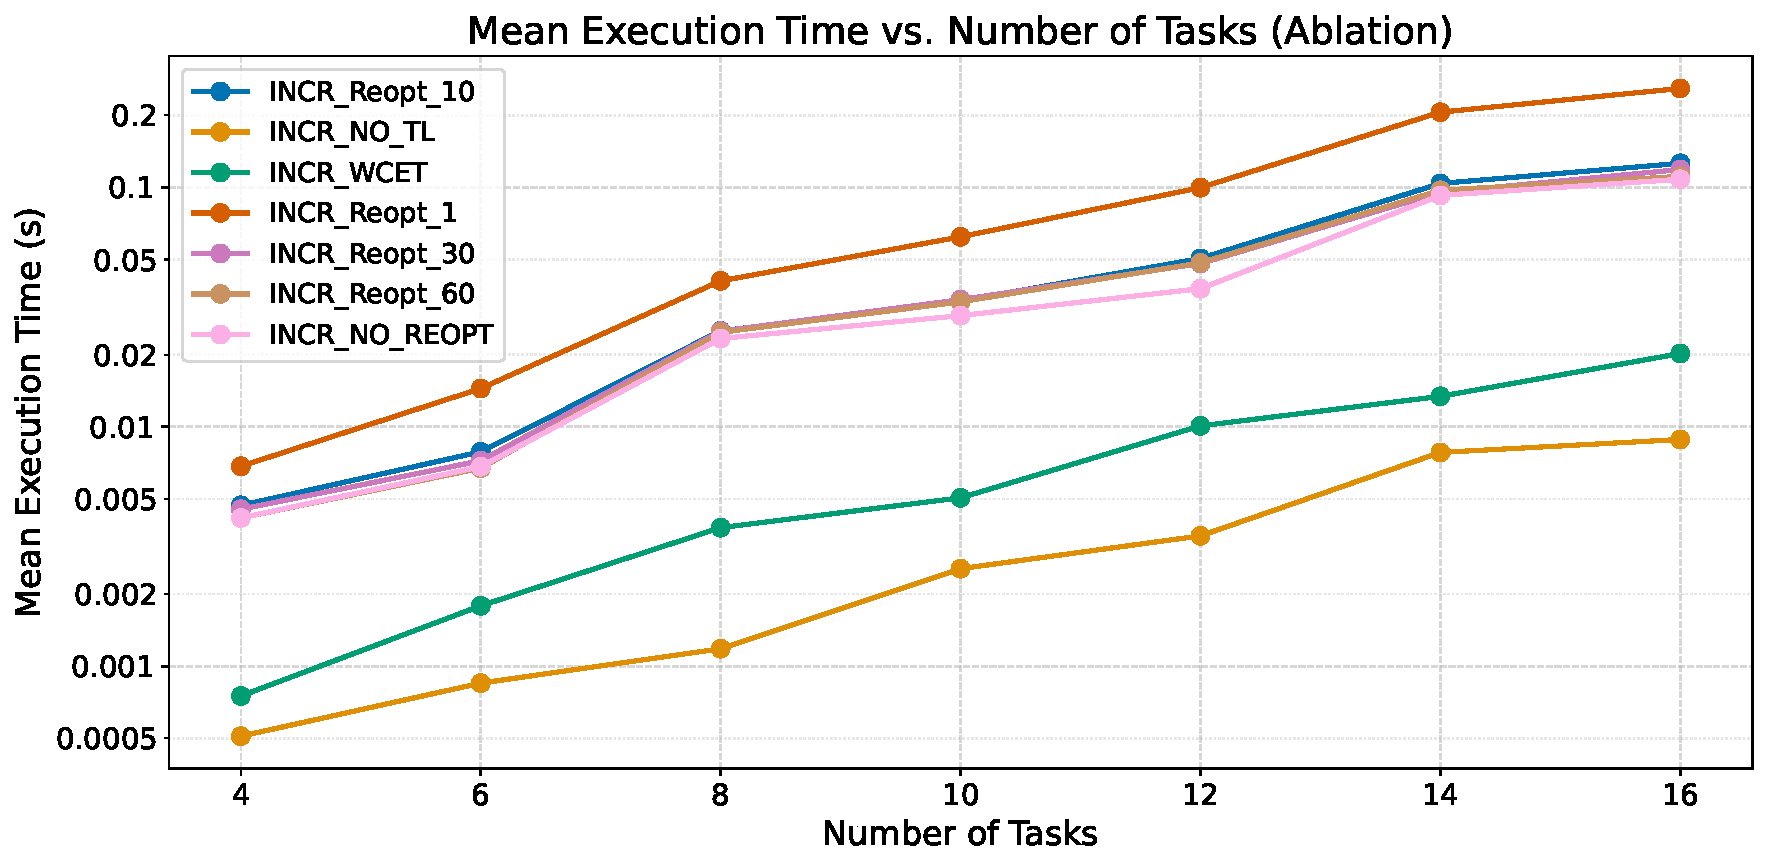
\includegraphics[width=\textwidth]{pictures/simulation/sim_ablation_exec_time.pdf}
        \caption{Optimizer execution time of ablation arms.}
        \label{fig_sim_ablation_exec}
    \end{subfigure}
    \caption{Ablation study ($N\in\{4,\dots,16\}$). QoS-budget optimization is the dominant mechanism;
    distribution-aware execution times and periodic re-optimization each add a measurable gain.}
    \label{figs_sim_ablation}
\end{figure*}

The ablation arms isolate the contribution of each mechanism (Fig.~\ref{fig_sim_ablation_sp}).
Disabling QoS-budget optimization (INCR\_NO\_TL) collapses SP to the DM\_FAST level
(e.g., $0.643$ vs.\ $0.747$ at $N{=}8$): QoS-budget optimization is the single largest contributor,
confirming that adapting any-time algorithm budgets to the current load is where the gains come from.
Replacing the execution-time distribution with its worst-case value (INCR\_WCET) consistently
lowers SP ($0.736$ vs.\ $0.747$ at $N{=}8$; $0.625$ vs.\ $0.666$ at $N{=}12$).
The reason is the interaction with the feasibility gate: a pessimistic execution time yields a pessimistic
response-time analysis, so the gate rejects larger QoS budgets as unsafe and the walk settles on smaller,
lower-SP budgets; the gap widens with $N$ as overload makes more candidates appear infeasible.
Disabling periodic re-optimization (INCR\_NO\_REOPT) gives a smaller loss ($0.660$ vs.\ $0.670$
at $N{=}16$): re-optimization periodically realigns the solution with the global optimum after incremental
drift (Section~\ref{sec: drift}).
Finally, sweeping the re-optimization period (INCR\_Reopt\_1/10/30/60) leaves SP nearly flat,
so the method is insensitive to this parameter within the tested range.

Fig.~\ref{fig_sim_ablation_exec} shows the optimizer execution time of the ablation arms.
INCR\_WCET is the cheapest because its pessimistic gate accepts fewer budget steps; more frequent
re-optimization (INCR\_Reopt\_1) costs more, while longer periods approach the pure-incremental cost.

QoS-budget optimization is the dominant source of improvement; using the execution-time distribution
rather than its worst-case bound is essential because the feasibility gate otherwise over-rejects; and
periodic re-optimization yields a modest but consistent gain at modest cost.

\subsection{Effectiveness of the Fallback Mechanism}
\label{section: sim_fallback}

\begin{figure}[!htbp]
    \centering
    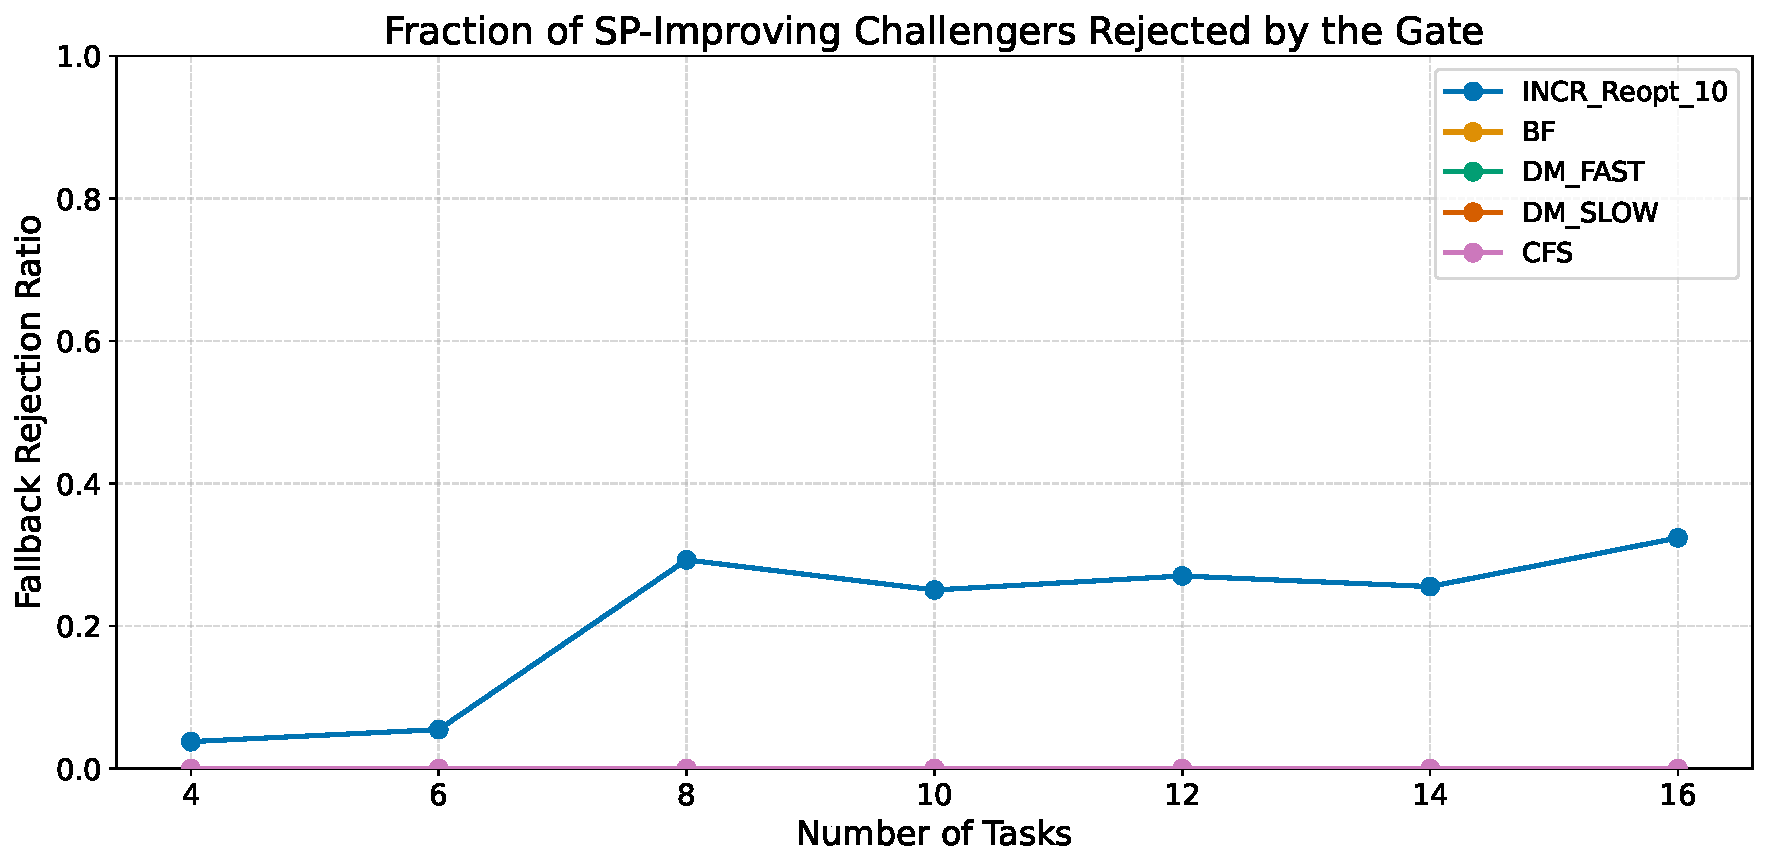
\includegraphics[width=\columnwidth]{pictures/simulation/sim_fallback_rejection.pdf}
    \caption{Fraction of scheduler invocations adopting the safe fallback.
    It remains low, engaging only when the inherited configuration becomes unschedulable.}
    \label{fig_sim_fallback}
\end{figure}

Fig.~\ref{fig_sim_fallback} reports the fraction of scheduler invocations in which the fallback
mechanism (Section~\ref{section_safety_fallback}) is adopted---that is, where the incremental walk would
otherwise terminate on an unschedulable incumbent under an execution-time jump or overload.
The fraction stays low across the full scale range, indicating that the walk ordinarily finds a
schedulable solution on its own; the fallback engages only in the rarer cases where the inherited
configuration becomes unreliable, and there it preserves important-task schedulability at a small SP
penalty.

The fallback protects safety-critical schedulability with negligible SP penalty, intervening only when
the incremental solution would otherwise be unsafe.
